\section{Client-Dispatcher-Server}


Das Client-Dispatcher-Server Design-Pattern führt eine Zwischenschicht zwischen Clients und Server ein, die Dispatcher-Komponente. Es stellt Orts-Transparenz (location transparency) in Form eines Namensdienstes (name service) zur Verfügung und versteckt die Details der Kommunikationsverbindung zwischen Client und Server.

\subsection*{Example}


Stellen wir uns vor wir würden ein Softwaresystem namens ACHILLES zum Empfangen von neuen, wissenschaftlichen Informationen entwickeln. Die Informations-Provider sind sowohl lokal in unserem Netzwerk, wie auch verteilt über die Welt. Es ist nötig den Ort und den auszuführenden Dienst zu spezifizieren. Empfängt ein Informations-Provider einen Request von einer Client-Anwendung führt er den entsprechenden Dienst aus und gibt die angefragte Informations dem Client zurück.

\subsection*{Context}


Ein Software-System integriert eine Menge von verteilten Servern, welche lokal oder verteilt über ein Netzwerk laufen.

\subsection*{Problem}


Benutzt ein Software System über ein Netzwerk verteilte Server muss es Mittel zur Kommunikation zwischen ihnen bereitstellen. In vielen Fällen muss eine Verbindung aufgebaut werden, bevor eine Kommunikations stattfinden kann, abhängig von der verwendeten Kommunikationsart. Die eigentliche Funktionalität der Komponenten soll jedoch von den Details des Kommunikations-Mechanismus getrennt sein. Clients sollen nicht wissen müssen wo sich die Server befinden. Dadurch lässt sich der Standardort der Server dynamisch anpassen und das System ist robust gegenüber Netzwerk oder Server ausfällen.

\subsubsection*{Forces}


\begin{itemize}
	\item Eine Komponente soll einen Dienst (Service) unabhängig vom Standarort des Service-Providers nutzen können
	\item Der Code welcher die Funktionalität des Service-Consumer implementiert soll getrennt sein vom Code welcher nötig ist um eine Verbindung aufzubauen.
\end{itemize}

\subsection*{Solution}


Stelle eine Dispatcher Komponente als Zwischenschicht zwischen Client und Server zur Verfügung. Der Dispatcher implementiert einen Namensdienst (name service) welcher es Clients erlaubt über einen Namen anstatt über den physikalischen Ort auf den Server anzupassen, wodurch eine Ortstransperenz zur Verfügung gestellt wird. Zudem ist der Dispatcher verantwortlich den Kommunikationskanal zwischen Client und Server aufzubauen.

Füge Server zur Anwendung hinzu welche Dienste anderen Komponenten anbieten. Jeder Server wird über einen eindeutigen Namen identifziert und ist über den Dispatcher mit Clients verbunden.

Clients benötigen den Dispatcher um ein bestimmten Server zu finden und einen Verbindung mit dem Server aufzubauen. Im Gegensatz zum traditionellem Client-Server Modell können die Rollen von Clients und Server dynamisch ändern.

\subsection*{Structure}

\begin{figure}[H]
	\centering
	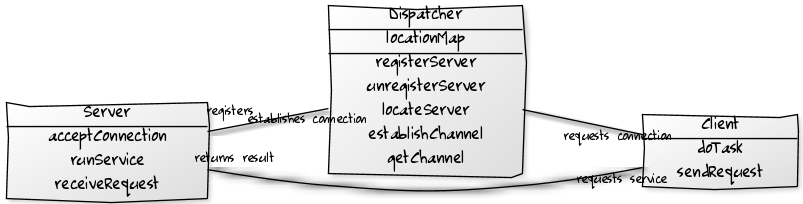
\includegraphics[width=0.7\textwidth]{content/posa1/images/client-dispatcher-server-classes.png}
	\caption{Client Dispatcher Server Klassendiagramm}
\end{figure}


Die Aufgabe eines Clients ist es domänenspezifische Aufgaben auszuführen. Der Client greift auf Operationen welche von Servern zur Verfügung gestellt werden zu um seine Aufgabe auszuführen. Bevor ein Request an einen Server gesendet wird, bittet der Client den Dispatcher um einen Kommunikationskanal. Der Client benutzt diesen Kanal um mit der Server zu kommunizieren.

Ein Server stellt eine Menge von Operationen den Clients zur Verfügung. Er ist beim Dispatcher mit seinem Namen und seiner Adresse registiert. Eine Server-Komponente kann sich auch auf dem selben Computer wie ein Client befinden oder über das Netzwerk erreichbar sein.

Der Dispatcher stellt Funktionalität zum Aufbau von Kommunikations-Kanälen zur Verfügung. Dazu nimmt er den Namen der Server Komponente und mappt den entsprechenden physikalischen Ort der Server Komponente. Der Dispatcher erstellt eine Verbindung zum Server mit dem zur Verfügung stehenden Kommunikationsmechanismus und gibt einen Kommunikations-Handle dem Client zurück. Falls der Dispatcher keine Verbindung mit dem entsprechenden Server aufbauen kann informiert er den Client über den Fehler.

Um den Namensdienst (name service) zur Verfügung zu stellen implementiert der Dispatcher Funktionen um Server zu registrieren und zu finden.

\subsection*{Dynamics}

\begin{figure}[H]
	\centering
	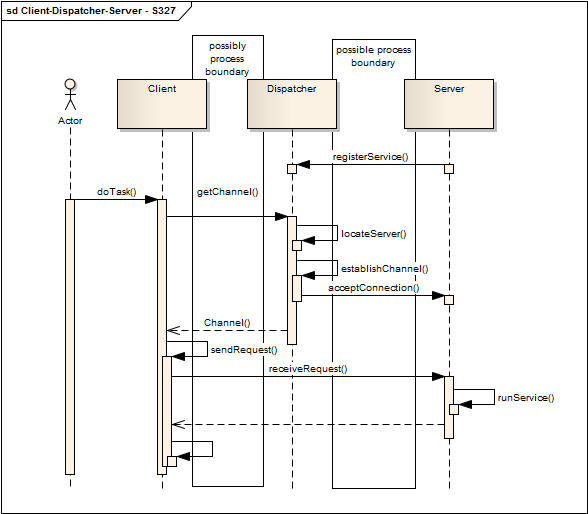
\includegraphics[width=0.7\textwidth]{content/posa1/images/client-dispatcher-server-sequence.png}
	\caption{Client Dispatcher Server Klassendiagramm}
\end{figure}

\begin{enumerate}
	\item png
	\item Ein Server registiert sich selbst bei der Dispatcher Komponente.
	\item Später bittet ein Client den Dispatcher um einen Kommunikationskanal mit einem bestimmten Server.
	\item Der Dispatcher sieht in seiner Registry nach welcher Server mit dem entsprechenden Namen registiert ist.
	\item Der Dispatcher erzeugt eine Kommunikations-Verbindung mit dem Server. Falls er die Verbindung erfolgreich herstellen kann gibt er den Kanal dem Client zurück. Falls nicht, sendet er einen Fehlermeldung.
	\item Der Client bentuzt den Kommunikationskanal um Requests direkt an den Server zu senden.
	\item Nachdem der Server einen eingehenden Request erkannt hat führt den den entsprechenden Dienst aus.
	\item Sobald der Dienst ausgeführt wurde sendet der Server das Resultat an den Client zurück.
\end{enumerate}

\subsection*{Implementation}
\begin{enumerate}
	\item Unterteile die Anwendung in Server und Clients. Server können möglicherweise vorgegeben sein und müssen integriert werden. Da Clients möglicherweise auch als Server fungieren können und umgekehrt sind die Rollen nicht Vordefiniert und können zur Laufzeit ändern.
	\item Entscheide welche Kommunikationsarten benötigt werden. Eine einzige Kommunikationsart vereinfacht die Komplexität der Implementation. Aus Performancegründen kann dies aber nicht immer angebracht sein. So kann falls der Client und der Server auf dem selben Rechner ausgeführt werden Shared-Memory die schnellste Art der Interprozesskommunikation sein. Falls bestehende Server in das System integriert werden sollen ist die Kommunikationsart durch diese Server möglicherweise vorgegeben.
	\item Spezifiziere die Interaktionsprotokolle zwischen Komponenten. Es sind drei Protokolle denkbar, ein Client-Server-Protokoll (CSProtocol), ein Client-Dispatcher-Protokoll (CDProtocol) und ein Dispatcher-Server-Protokoll (DSProtocol).
	\item Entscheide wie die Server genannt werden. Die Namen sollen eindeutig und unabhängig vom Ort der Server sein.
	\item Designe und implementiere den Dispatcher. Limitierte Resourcen (anzahl Sockets) und Performance-Probleme sollen dabei besonders beachtet werden.
	\item Implementiere die Client und Server Komponenten.
\end{enumerate}


\begin{itemize}
	\item Distributed Dispatchers: Statt einen einzelnen Dispatcher können verteilte Dispatcher eingesetzt werden. Dabei kann ein lokaler Dispatcher einen entfernten Dispatcher anfragen oder Clients können direkt mit entfernten Dispatcher kommunizieren. Möglicherweise ist das Broker Pattern dem einsatz von Distrubuted Dispatchern vorzuziehen.
	\item Client-Dispatcher-Server with communication managed by clients: Dabei fungiert der Dispatcher als Namensdienst und überlässt den Verbindungsaufbau dem Client.
	\item Client-Dispatcher-Server with heterogeneous communication: Manchmal kann die Kommunikation von Clients und Servern nicht über ein einziges Kommunikationsprotokoll abgewickelt werden, zum Beispiel wenn verschiedene bestehende Server verschiedene Kommunikationsmechansimen benötigen. Der Dispatcher muss dann mehrere Kommunikationsmechanismen unterstützen.
	\item Client-Dispatcher-Service: Dabei werden die Services Adressiert und nicht die Server. Bekommt der Dispatcher einen Request schaut er nach welcher Server den entsprechenden Service bereitstellt und stellt die Verbindung zum entsprechenden Serivce-Provider bereit.
\end{itemize}

\subsection*{Known Uses}


\begin{itemize}
	\item Remote Procedure Calls
	\item OMG Corba
\end{itemize}

\subsection*{Consequences}


\subsubsection*{Benefits}


\begin{itemize}
	\item Austauschbarkeit der Server: Server können ohne Änderungen an der Dispatcher-Komponente ausgetauscht werden.
	\item Orts- und Migrationstransparenz: Clients müssen den Ort der Server nicht können und die Dienste können dynamisch auf andere Rechner migiert werden.
	\item Re-Konfiguration: Wo sich die Server befinden kann zur Laufzeit entschieden werden. Das Client-Dispatcher Pattern ermöglicht es auch ein Software System zu entwerfen welches erst später in eine verteilte Anwendung überführt wird.
	\item Fault tolerance: Server können auch auf weiteren Netzwerk-Knoten aktiviert werden ohne dass dies einen Einfluss auf die Clients hat. Das System ist dadurch robuster und fault-toleranter.
\end{itemize}

\subsubsection*{Liablities}


\begin{itemize}
	\item Geringere Effizienz durch Indirektion und explizitem Verbindungsaufbau.
	\item Empfindlich auf Änderungen der Schnittstelle der Dispatcher-Komponente.
\end{itemize}

\subsection*{See also}


\begin{itemize}
	\item Forwarder-Receiver Pattern, lässt sich mit dem Client-Dispatcher-Server Pattern kombinieren
	\item Acceptor and Connector Patterns(Doug Schmidt), zeigen einen anderen Weg um den Verbindungsaufbau von der Verarbeitung zu trennen. Schmidts Pattern sind dezentralisierter. Alles was Verbindungen akzeptiert kann eine Familie von Acceptor-Factories bereitstellen. Diese Acceptors sind verantwortlich Service-Handlers zu konstruieren.
\end{itemize}
